\documentclass[12pt]{article}
\usepackage{graphicx,import}
\usepackage{float}
\usepackage[svgnames]{xcolor} 
\usepackage{fancyhdr}
\usepackage{subcaption}
\usepackage{hyperref}
\usepackage{enumitem}
\usepackage{cite}
\usepackage[many]{tcolorbox}
\usepackage{listings }
\usepackage[a4paper, total={6in, 8in} , bottom = 25mm , top = 25mm, headheight = 1.25cm , includehead,includefoot,heightrounded ]{geometry}
\usepackage{afterpage}
\usepackage{amssymb}
\usepackage{pdflscape}
\usepackage{gensymb}
\usepackage{textcomp}
\usepackage{tikz,pgfplots}
\usepackage{xecolor}
\usepackage{rotating}
\usepackage{pdfpages}
\usepackage[Kashida]{xepersian}
\usepackage[T1]{fontenc}
\usepackage{tikz}
\usepackage[utf8]{inputenc}
\usepackage{PTSerif} 
\usepackage{seqsplit}
\usepackage{url}

\usepackage[edges]{forest}

\usepackage{listings}
\usepackage{xcolor}

\hypersetup{
	colorlinks   = true, %Colours links instead of ugly boxes
	urlcolor     = blue, %Colour for external hyperlinks
	linkcolor    = blue, %Colour of internal links
	citecolor   = red %Colour of citations
}
 
\definecolor{codegreen}{rgb}{0,0.6,0}
\definecolor{codegray}{rgb}{0.5,0.5,0.5}
\definecolor{codepurple}{rgb}{0.58,0,0.82}
\definecolor{backcolour}{rgb}{0.95,0.95,0.92}
 
\NewDocumentCommand{\codeword}{v}{
\texttt{\textcolor{blue}{#1}}
}
\lstset{language=java,keywordstyle={\bfseries \color{blue}}}


\lstdefinestyle{mystyle}{
    backgroundcolor=\color{backcolour},   
    commentstyle=\color{codegreen},
    keywordstyle=\color{magenta},
    numberstyle=\tiny\color{codegray},
    stringstyle=\color{codepurple},
    basicstyle=\ttfamily\normalsize,
    breakatwhitespace=false,         
    breaklines=true,                 
    captionpos=b,                    
    keepspaces=true,                 
    numbers=left,                    
    numbersep=5pt,                  
    showspaces=false,                
    showstringspaces=false,
    showtabs=false,                  
    tabsize=2
}

\lstset{style=mystyle}

\settextfont[Scale=1.2 ,BoldFont={Bahij Nazanin-Bold.ttf} , ItalicFont = {IRNazaninIranic.ttf}]{Bahij Nazanin-Regular.ttf}
\setlatintextfont[Scale = 1.0]{Garamond}
\DefaultMathsDigits 
\DeclareMathSizes{11}{19}{13}{9} 
%\DeclareMathSizes{12}{14.4}{8}{9}





\newenvironment{changemargin}[2]{%
\begin{list}{}{%
\setlength{\topsep}{0pt}%
\setlength{\leftmargin}{#1}%
\setlength{\rightmargin}{#2}%
\setlength{\listparindent}{\parindent}%
\setlength{\itemindent}{\parindent}%
\setlength{\parsep}{\parskip}%
}%
\item[]}{\end{list}}


\definecolor{foldercolor}{RGB}{124,166,198}

\tikzset{pics/folder/.style={code={%
    \node[inner sep=0pt, minimum size=#1](-foldericon){};
    \node[folder style, inner sep=0pt, minimum width=0.3*#1, minimum height=0.6*#1, above right, xshift=0.05*#1] at (-foldericon.west){};
    \node[folder style, inner sep=0pt, minimum size=#1] at (-foldericon.center){};}
    },
    pics/folder/.default={20pt},
    folder style/.style={draw=foldercolor!80!black,top color=foldercolor!40,bottom color=foldercolor}
}

\forestset{is file/.style={edge path'/.expanded={%
        ([xshift=\forestregister{folder indent}]!u.parent anchor) |- (.child anchor)},
        inner sep=1pt},
    this folder size/.style={edge path'/.expanded={%
        ([xshift=\forestregister{folder indent}]!u.parent anchor) |- (.child anchor) pic[solid]{folder=#1}}, inner xsep=0.6*#1},
    folder tree indent/.style={before computing xy={l=#1}},
    folder icons/.style={folder, this folder size=#1, folder tree indent=3*#1},
    folder icons/.default={12pt},
}

\begin{document}


%%% title pages
\begin{titlepage}
\begin{center}
        
\vspace*{0.7cm}


\includegraphics[width=0.4\textwidth]{sharif1.png}\\
\vspace{0.5cm}
\textbf{ \Huge{\emph ‌آزمایشگاه شبکه‌های کامپیوتری} }\\
\vspace{0.5cm}
\textbf{ \Large{ آزمایش پنجم} }
\vspace{0.2cm}
       
 
      \large \textbf{دانشکده مهندسی کامپیوتر}\\\vspace{0.2cm}
    \large   دانشگاه صنعتی شریف\\\vspace{0.2cm}
       \large   ﻧﯿﻢ سال دوم 01-00 \\\vspace{0.2cm}
      \noindent\rule[1ex]{\linewidth}{1pt}
استاد:\\
    \textbf{{جناب آقای دکتر صفایی}}


    \vspace{0.15cm}
اعضای گروه:\\

    \textbf{{محمدسپهر پورقناد - 97101359}}
    \\
   
    \textbf{{سپهر صفری - 97108263}}       
   \\
   
    \textbf{{امیرمهدی نامجو - 97107212}}
\end{center}
\end{titlepage}
%%% title pages


%%% header of pages
\newpage
\pagestyle{fancy}
\fancyhf{}
\fancyfoot{}
\cfoot{\thepage}
\chead{}
\rhead{
\includegraphics[width=0.1\textwidth]{sharif.png}}
\lhead{آزمایش پنجم}
%%% header of pages

\newfontfamily\terminal{Courier New Bold}

\KashidaOff
 \newcommand{\inlineLatin}[1]{
	\small{\lr{{\terminal #1}}}
}

توجه: فایل‌های \inlineLatin{ospf.pkt} و \inlineLatin{rip.pkt} در فایل \inlineLatin{zip} ارسالی قرار دارند.

\section{RIP}

در این آزمایش هدف ما راه‌اندازی الگوریتم مسیر‌یابی \inlineLatin{RIP} است. ابتدا مطابق تصویر داده شده در صورت سوال، روترها و \inlineLatin{PC}‌ ها را قرار می‌دهیم.

\begin{figure}[H]
	\centering
	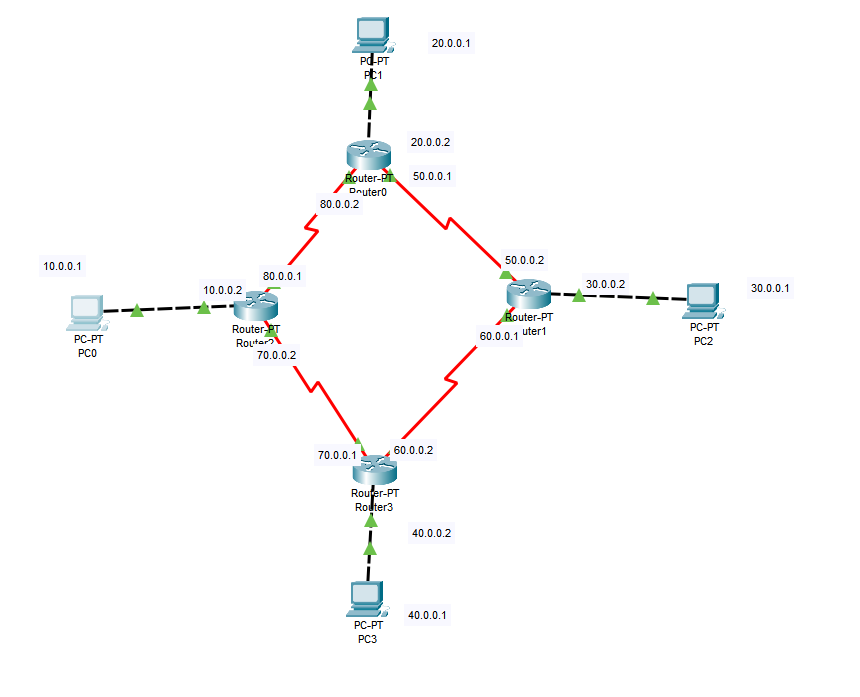
\includegraphics[scale=0.4]{images/rip/8.png}
	\caption{توپولوژی داده شده در صورت سوال} 
	\label{topology}
\end{figure}

در شکل بالا، آی‌پی‌های اختصاص داده شده به هر بخش هم مشخص است ولی برای واضح‌تر شدن کار،‌ تنظیمات اعمال شده برای یکی از \inlineLatin{PC} ها و یکی از روترها در شکل‌های زیر آمده است.

تنظیمات مربوط به \inlineLatin{Router2}:
\begin{figure}[H]
	\centering
	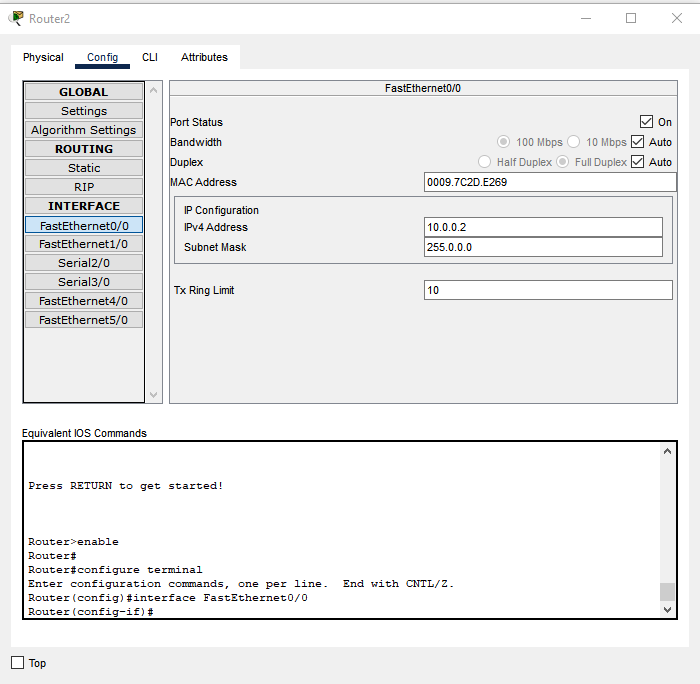
\includegraphics[scale=0.4]{images/rip/1.png}
	\caption{اتصال بین \inlineLatin{Router2} و \inlineLatin{PC0}} 
	\label{r2pc0}
\end{figure}


\begin{figure}[H]
	\centering
	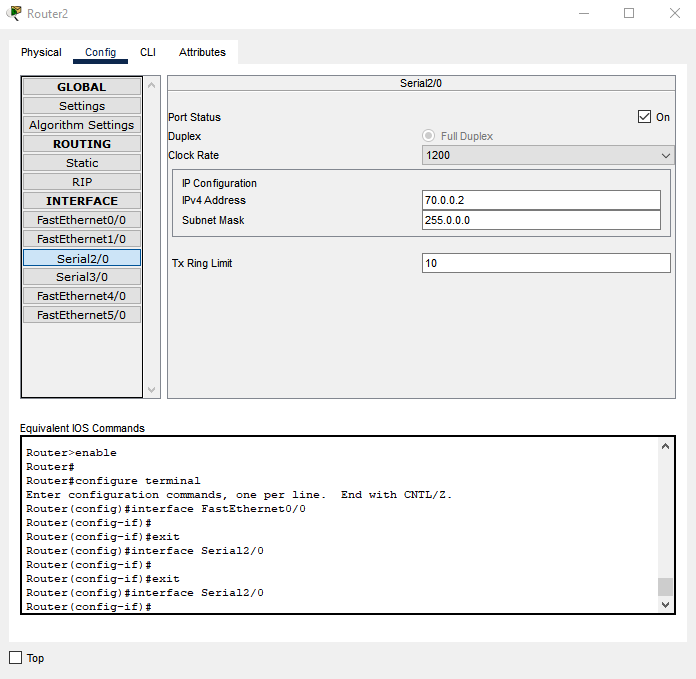
\includegraphics[scale=0.4]{images/rip/2.png}
	\caption{اتصال بین \inlineLatin{Router2} و \inlineLatin{Router3}} 
	\label{r2r3}
\end{figure}


\begin{figure}[H]
	\centering
	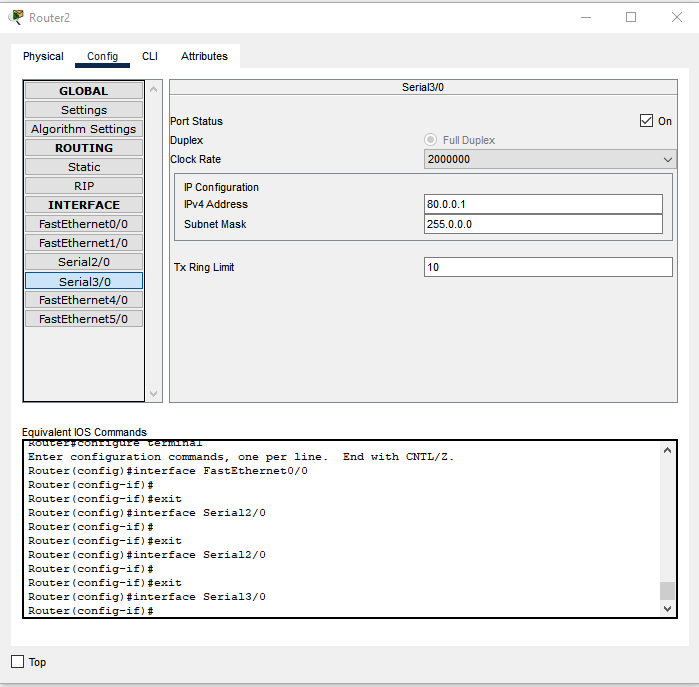
\includegraphics[scale=0.4]{images/rip/3.png}
	\caption{اتصال بین \inlineLatin{Router2} و \inlineLatin{Router0}} 
	\label{r2r0}
\end{figure}

تنظیمات مربوط به \inlineLatin{PC0}:


\begin{figure}[H]
	\centering
	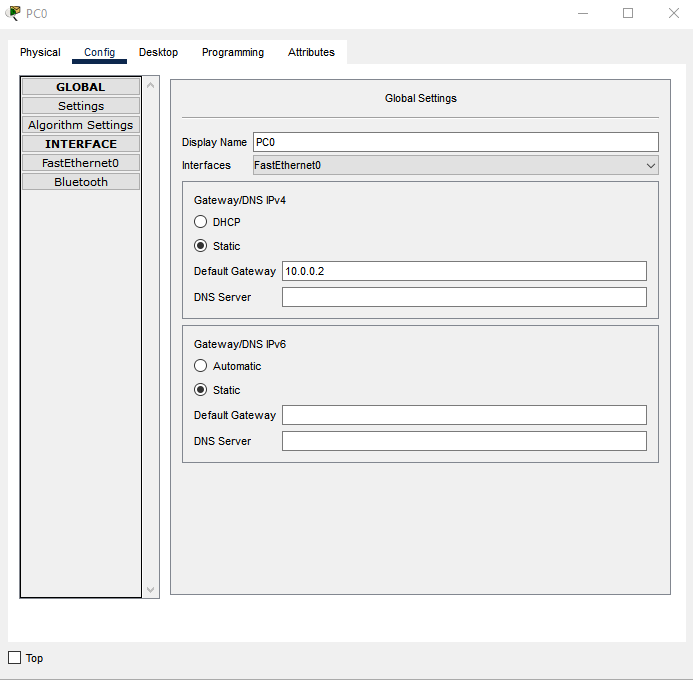
\includegraphics[scale=0.4]{images/rip/5.png}
	\caption{تنظیم \inlineLatin{Default Gateway}} 
	\label{defaultgatewayconfig}
\end{figure}

\begin{figure}[H]
	\centering
	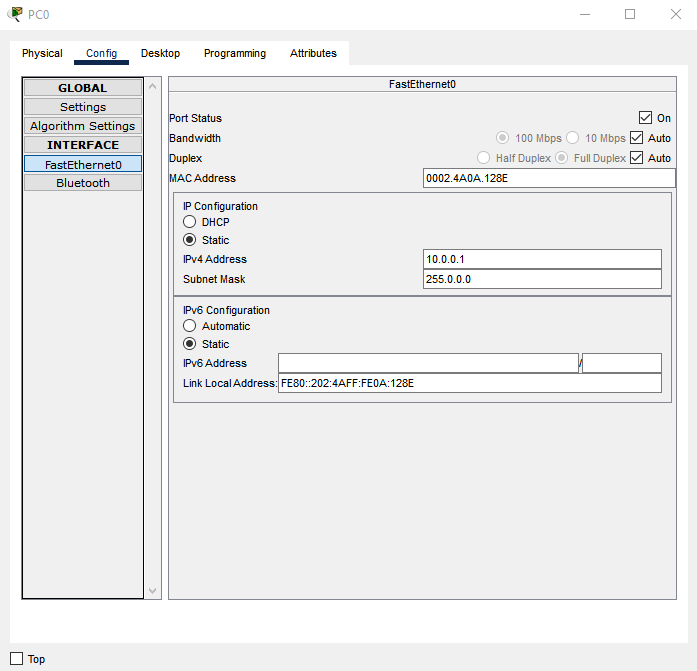
\includegraphics[scale=0.4]{images/rip/6.png}
	\caption{تنظیم \inlineLatin{IP}} 
	\label{configip}
\end{figure}

سپس تنظیمات مربوط به \inlineLatin{RIP} را در روترها وارد می‌کنیم. به عنوان نمونه تنظیمات مربوط به \inlineLatin{Router2} در زیر قرار گرفته است:

\begin{figure}[H]
	\centering
	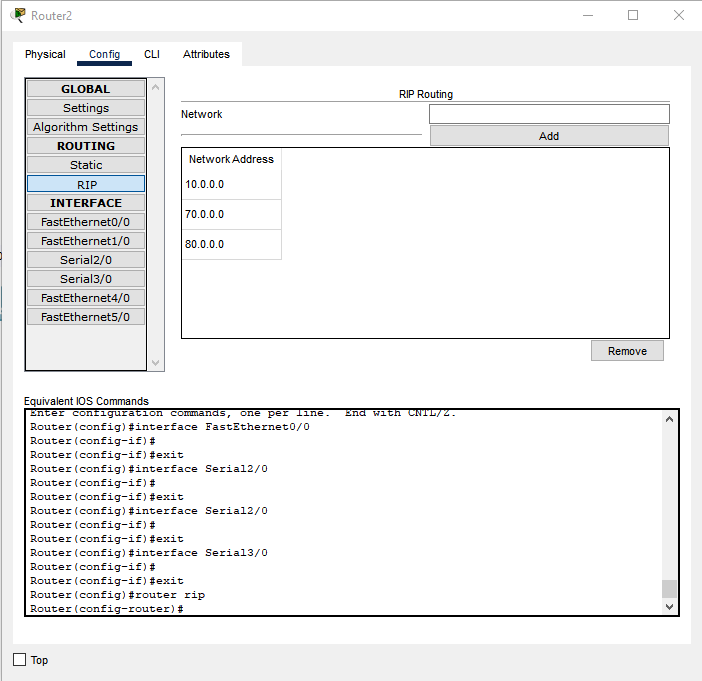
\includegraphics[scale=0.4]{images/rip/4.png}
	\caption{تنظیم \inlineLatin{RIP} در \inlineLatin{Router2}} 
	\label{ripr2}
\end{figure}

بعد از اعمال تنظیمات، به خوبی اتصال‌ها برقرار شده و در زیر نمونه‌ای از اجرای دستور \inlineLatin{ping} و \inlineLatin{tracert} را برای \inlineLatin{PC0} مشاهده می‌کنید.

\begin{figure}[H]
	\centering
	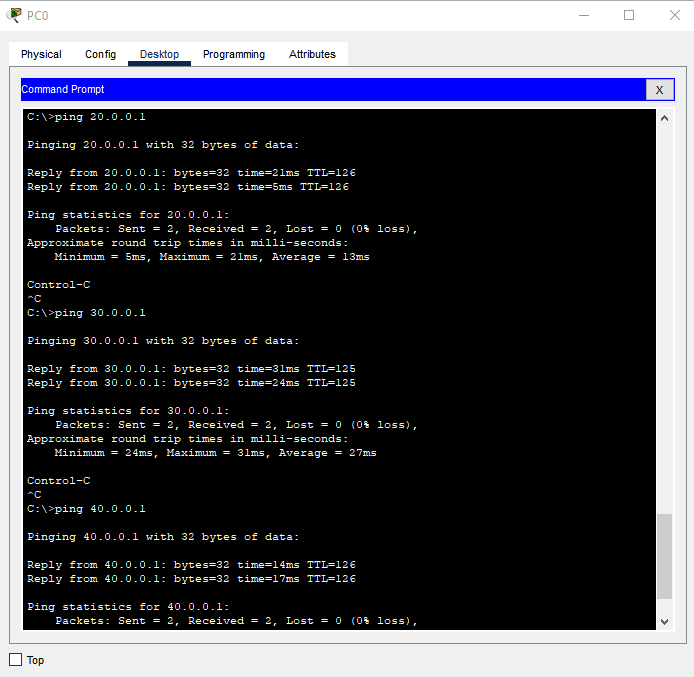
\includegraphics[scale=0.4]{images/rip/7.png}
	\caption{اجرای دستور \inlineLatin{ping} در \inlineLatin{PC0}} 
	\label{ripping}
\end{figure}

\begin{figure}[H]
	\centering
	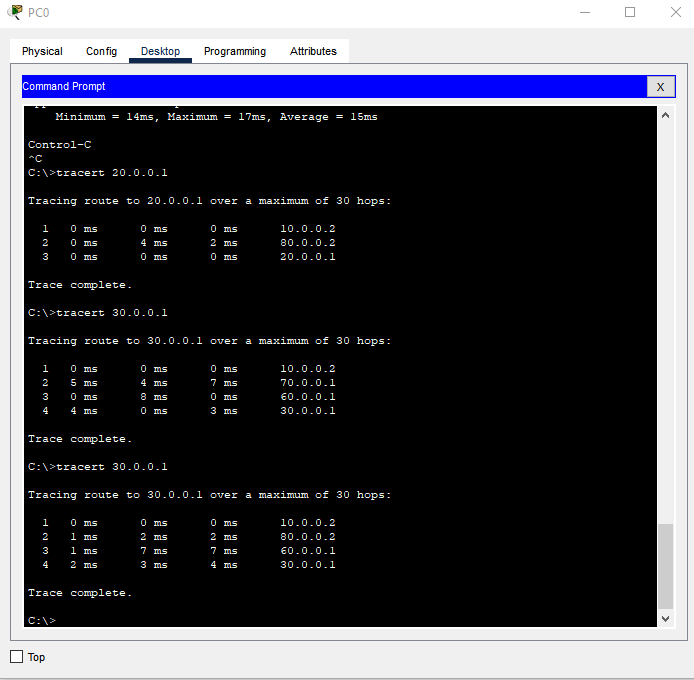
\includegraphics[scale=0.4]{images/rip/9.png}
	\caption{اجرای دستور \inlineLatin{tracert} در \inlineLatin{PC0}} 
	\label{showiprip}
\end{figure}


و همچنین نتیجه اجرای دستور
\inlineLatin{show ip route}
در \inlineLatin{Router2} به صورت زیر است.

\begin{figure}[H]
	\centering
	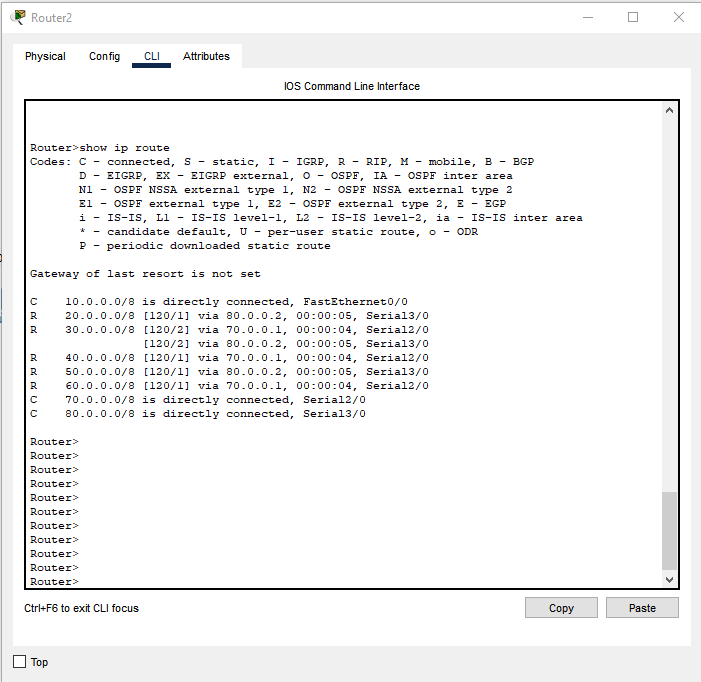
\includegraphics[scale=0.4]{images/rip/10.png}
	\caption{اجرای دستور \inlineLatin{show ip route} در \inlineLatin{Router2}} 
	\label{showiprip2}
\end{figure}

همچنین در شکل زیر بخشی از اطلاعاتی که برای یک پکت \inlineLatin{Sniff} شده \inlineLatin{RIP} توسط نرم‌افزار نشان داده می‌شود را مشاهده می‌کنید.

\begin{figure}[H]
	\centering
	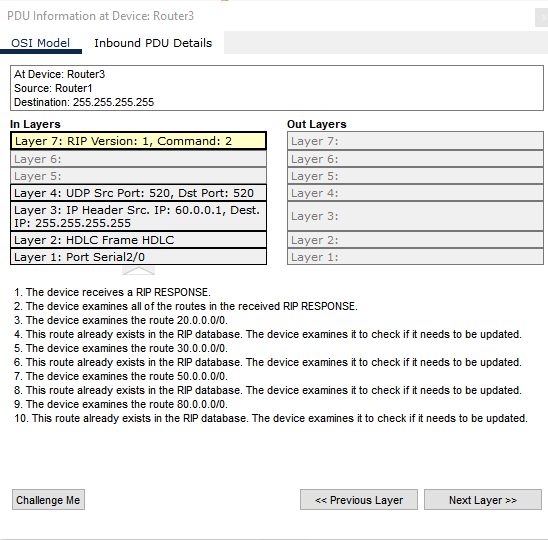
\includegraphics[scale=0.4]{images/rip/RipSniff.png}
	\caption{پکت \inlineLatin{Sniff} شده \inlineLatin{RIP}} 
	\label{ripsniff}
\end{figure}

\newpage

\section{OSPF}

\subsection{سوالات}


برای پاسخ به این قسمت سه مورد را بررسی می‌کنیم.

\begin{itemize}
	\item انواع روتر در OSPF
	
	\item پکت‌های LSA
	
	\item انواع Area ها
	
	
\end{itemize}


\subsubsection{انواع روتر در OSPF}

\begin{itemize}
	\item \inlineLatin{Backbone Router}
	روتری که حداقل یک اینترفیس در ناحیه صفر داشته باشد.
	
	\item 
	\inlineLatin{Inline Router}
	روتری که همه اینترفیس‌هایش در یک ناحیه باشد.
	
	\item 
	\inlineLatin{Area Border Router (ABR)}
	روتری که یک یا چند اینترفیس در ناحیه صفر و یک یا چند روتر در نواحی غیرصفر دارد.
	
	\item 
	\inlineLatin{Autonomous System Border Router (ASBR)}
	روتری که به یک ناحیه و همچنین به یک \inlineLatin{AS} خارجی متصل هستند و در عین حال به یک ناحیه OSPF هم متصل است. 
\end{itemize}

\subsubsection{انواع LSA}

کلمه LSA مخفف
\inlineLatin{Link State Advertisement}
است و بسته‌هایی است که هر روتر \inlineLatin{OSPF} به کمک آن مسیر‌های خود را تبلیغ می‌کند.

هفت نوع بسته \inlineLatin{LSA} وجود دارد.

\begin{enumerate}
	\item نوع اول یا نوع \inlineLatin{Router}: این بسته‌ها توسط هر روتر داخلی در یک ناحیه و به ازای هر لینک درون ناحهی تولید می‌شوند و تنها در یک ناحیه پخش می‌شوند.
	
	\item نوع دو یا نوع \inlineLatin{Network}: توسط \inlineLatin{Designated Router} که تک روتر اصلی انتخاب شده در هر شبکه برای ارتباطات \inlineLatin{OSPF} است ایجاد می‌شود. این نوع بسته فقط در یک ناحیه منتقل می‌شود.
	
	
	\item نوع سوم یا 
	\inlineLatin{Network Summary}:
	این نوع توسط \inlineLatin{ABR} ها و بین نواحی منتقل می‌شود.
	
	\item نوع چهار یا
	\inlineLatin{ASBR Summary}:
	این نوع برخلاف نامش توسط \inlineLatin{ABR} ها تولید شده و مسیر منتهی به \inlineLatin{ASBR} را مشخص می‌کند.
	
	\item نوع پنجم یا \inlineLatin{AS External}
	این نوع توسط \inlineLatin{ASBR} تولید شده و بازتوزیع مسیر‌هایی که توسط یک AS خارجی به OSPF اعلام شده است را مشخص  می‌کند.
	
	\item نوع ششم: این نوع برای \inlineLatin{Multicast OSPF} طراحی شده ولی خیلی کم استفاده می‌شود و در روترهای \inlineLatin{Cisco} از آن پشتیبانی نمی‌شود.
	
	\item نوع هفتم یا \inlineLatin{NSSA External}:
توسط \inlineLatin{ASBR} ها و در نواحی
\inlineLatin{Not-so-stubby}
تولید شده و از یک 
\inlineLatin{ASBR}
به
\inlineLatin{ABR}
رسیده و در \inlineLatin{ABR} تبدیل به نوع پنجم شده و در شبکه پخش می‌شود.

\end{enumerate}

\subsubsection{انواع Area}
\begin{itemize}
	\item ناحیه \inlineLatin{Backbone}: این ناحیه هسته اصلی شبکه \inlineLatin{OSPF} است و همه نواحی باید به نوعی به این ناحیه متصل باشند. به این ناحیه ناحیه صفر هم گفته می‌شود. این ناحیه از بسته‌های نوع ۱ تا ۵ استفاده می‌کند.
	
	\item نواحی \inlineLatin{Standard}:
	نواحی‌ای که در دسته‌های بعدی قرار نگیرند در این دسته هستند. خود ناحیه \inlineLatin{Backbone} هم در این دسته قرار می‌گیرد. این ناحیه از بسته‌های نوع ۱ تا ۵ استفاده می‌کند.
	
	\item ناحیه \inlineLatin{Stub}:
	در نواحی \inlineLatin{Stub} مسیر‌های خارجی درون شبکه از طریق ABR منتشر نمی‌شوند بلکه به جای آن‌ها یک مسیر پیش‌فرض منتشر انتشار می‌یابد. این ناحیه از بسته‌های نوع ۱ تا ۳ استفاده می‌کند.
	
	\item ناحیه \inlineLatin{Totally Stubby}:
	این ناحیه شبیه ناحیه قبل است با این تفاوت که پیام‌های نوع 3 را هم (به جز در حالتی خاص) دریافت نمی‌کند. این ناحیه از بسته‌های نوع ۱ و ۲ استفاده می‌کند.
	
	\item ناحیه \inlineLatin{Not-so-Stubby}:
	این ناحیه مشابه ناحیه \inlineLatin{Stub} است ولی یک روتر \inlineLatin{ASBR} هم در آن وجود دارد. این ناحیه از بسته‌های نوع ۱ تا ۳ و همچنین ۷ استفاده می‌کند.
\end{itemize}


منبع: \url{https://www.packetcoders.io/ospf-areas-explained/}
\subsection{آزمایش}

شکل زیر شماتیک کلی تقسیم‌بندی نواحی را برای این بخش نشان می‌دهد.

\begin{figure}[H]
	\centering
	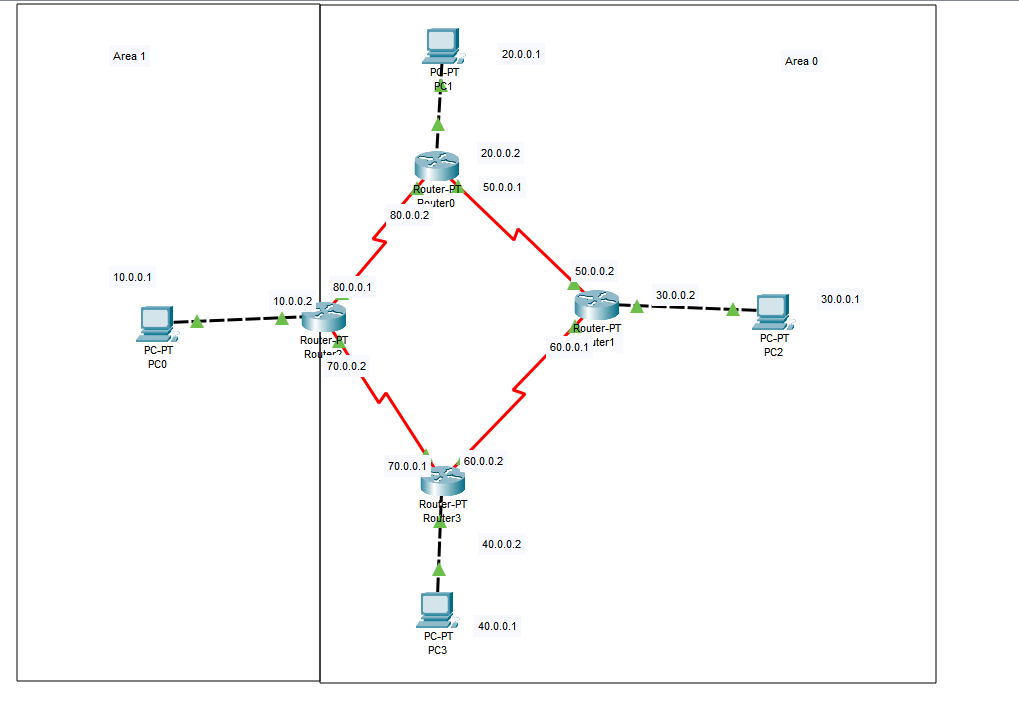
\includegraphics[scale=0.4]{images/ospf/topo.png}
	\caption{تقسیم‌بندی نواحی \inlineLatin{OSPF}} 
	\label{ospftopo}
\end{figure}

ابتدا تنظیمات مربوط به \inlineLatin{RIP} را پاک کرده و سپس تنظیمات مربوط به \inlineLatin{OSPF} را در روتر‌ها وارد می‌کنیم. ناحیه برای همه  ارتباطات روترها به جز \inlineLatin{Router2} صفر است ولی برای این روتر، برای ارتباطی که با \inlineLatin{PC0} دارد باید ناحیه را یک وارد کنیم.  توجه کنید که \inlineLatin{Router2} در توپولوزی‌ که من ایجاد کرده‌ام معادل \inlineLatin{R1} در شکل داده شده در صورت آزمایش است.

به عنوان نمونه تنظیمات وارد شده در \inlineLatin{Router2} در زیر قرار گرفته است:

\begin{figure}[H]
	\centering
	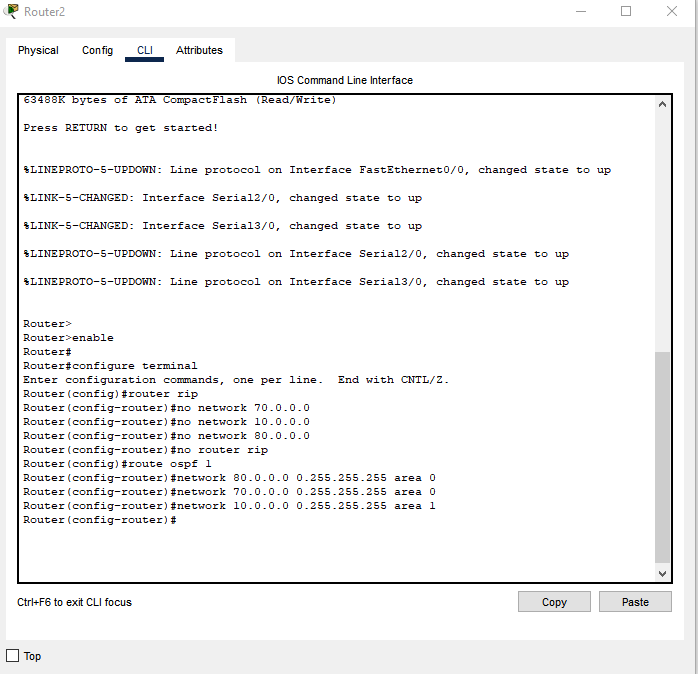
\includegraphics[scale=0.4]{images/ospf/15.png}
	\caption{تنظیمات وارد شده در \inlineLatin{Router2} برای \inlineLatin{OSPF}} 
	\label{riptracert}
\end{figure}

پس از انجام این کار در سایر روترها و انتقال پکت‌های OSPF، شاهد برقراری درست اتصال هستیم. در شکل‌های زیر حاصل دستور
\inlineLatin{show ip route}
برای 
\inlineLatin{Router0}
و
\inlineLatin{Router2}
نمایش داده شده است.

\begin{figure}[H]
	\centering
	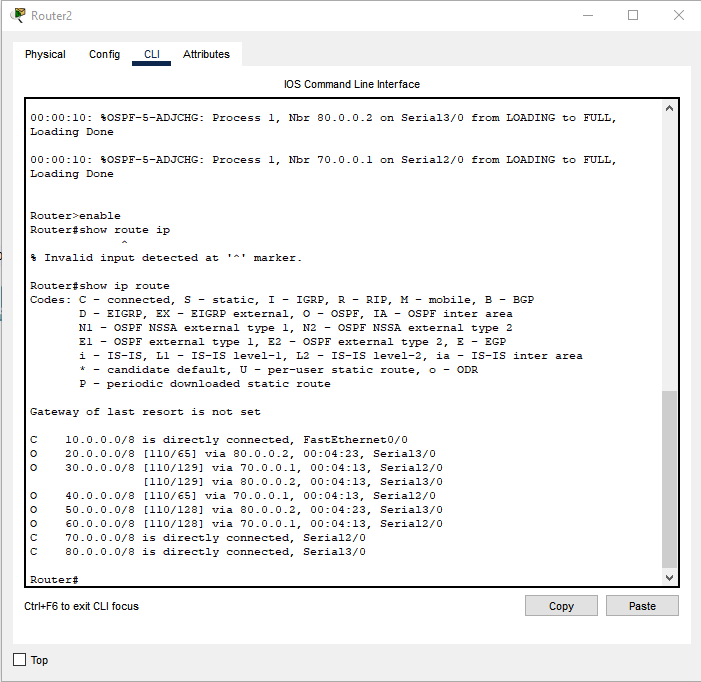
\includegraphics[scale=0.4]{images/ospf/13.png}
	\caption{اجرای دستور \inlineLatin{show ip route} در \inlineLatin{Router2}} 
	\label{iprouteospf}
\end{figure}

\begin{figure}[H]
	\centering	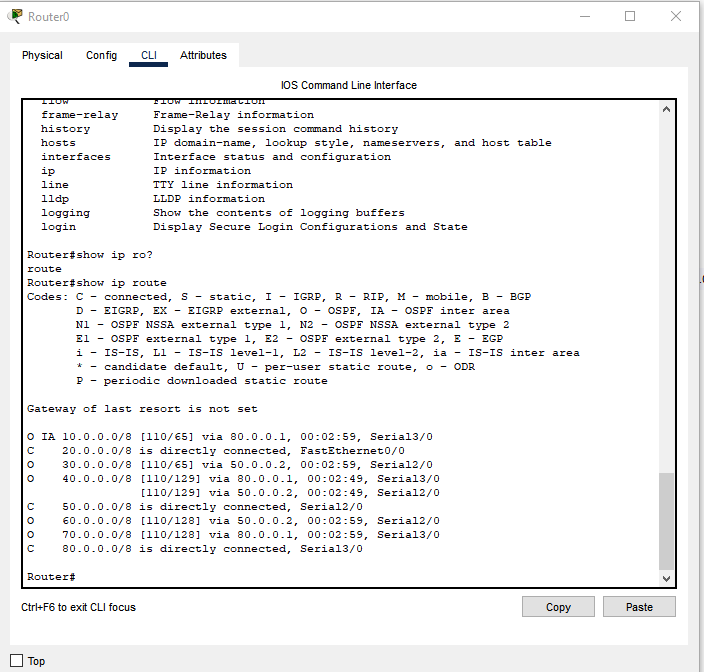
\includegraphics[scale=0.4]{images/ospf/12.png}
	\caption{اجرای دستور \inlineLatin{show ip route} در \inlineLatin{Router0}} 
	\label{iprouteospf2}
\end{figure}

همچنین نتیجه اجرای دستور \inlineLatin{tracert} در \inlineLatin{PC0} را در زیر مشاهده می‌کنید.

\begin{figure}[H]
	\centering
	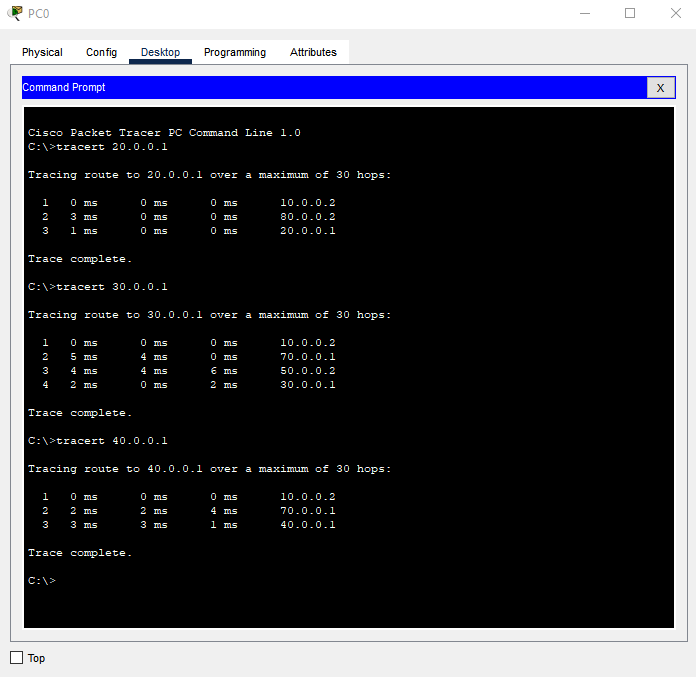
\includegraphics[scale=0.4]{images/ospf/14.png}
	\caption{اجرای دستور \inlineLatin{tracert} در \inlineLatin{PC0}} 
	\label{ospftracert}
\end{figure}

همچنین نمونه‌ای از یک پکت \inlineLatin{Sniff} شده \inlineLatin{OSPF} را در شکل زیر مشاهده می‌کنید.

\begin{figure}[H]
	\centering
	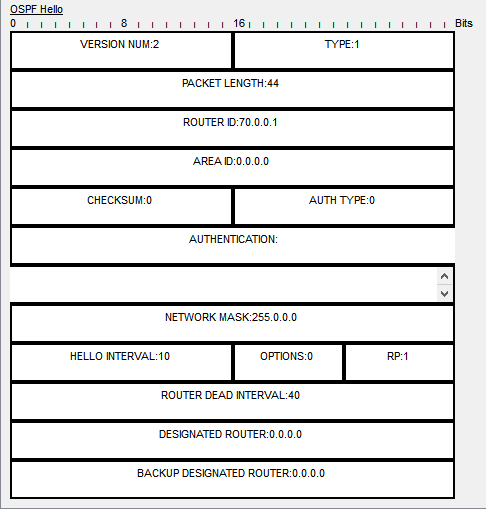
\includegraphics[scale=0.4]{images/ospf/11.png}
	\caption{پکت \inlineLatin{Sniff} شده \inlineLatin{OSPF}} 
	\label{ospfsniff}
\end{figure}


\end{document}



